% Pengaturan ukuran teks dan bentuk halaman dua sisi
\documentclass[12pt]{report}

% Pengaturan ukuran halaman dan margin
\usepackage[a4paper,top=30mm,left=30mm,right=20mm,bottom=25mm]{geometry}

% Pengaturan ukuran spasi
\usepackage[singlespacing]{setspace}

% Pengaturan caption untuk tabel
\usepackage{caption}

% Judul dokumen
\title{Proposal Tugas Akhir ITS}
\author{Musk, Elon Reeve}

% Pengaturan detail pada file PDF
\usepackage[pdfauthor={\@author},bookmarksnumbered,pdfborder={0 0 0}]{hyperref}


% Pengaturan ukuran indentasi
\setlength{\parindent}{2em}

% Package lainnya
\usepackage{changepage}
\usepackage{etoolbox} % Mengubah fungsi default

% Pengaturan jenis karakter
\usepackage[utf8]{inputenc}

\usepackage[style=apa, backend=biber]{biblatex}
\usepackage{enumitem} % Pembuatan list
\usepackage{lipsum} % Pembuatan template kalimat
\usepackage{graphicx} % Input gambar
\usepackage{longtable} % Pembuatan tabel
\usepackage[table,xcdraw]{xcolor} % Pewarnaan tabel
\usepackage{eso-pic} % Untuk menggunakan background image di halaman
\usepackage{txfonts} % Font times
\usepackage{changepage} % Pembuatan teks kolom
\usepackage{multicol} % Pembuatan kolom ganda
\usepackage{multirow} % Pembuatan baris ganda
\usepackage{tabularx} % Untuk mengatur kolom, seperti grid pada CSS
\usepackage{wrapfig}

% Pengaturan format daftar isi, daftar gambar, dan daftar tabel
\usepackage{tocloft}
\setlength{\cftbeforechapskip}{1.5ex}
\setlength{\cftbeforesecskip}{1.5ex}
\setlength{\cftbeforetoctitleskip}{0cm}
\setlength{\cftbeforeloftitleskip}{0cm}
\setlength{\cftbeforelottitleskip}{0cm}
\renewcommand{\cfttoctitlefont}{\hfill\Large\bfseries} % command untuk membuat heading bold dan besar
\renewcommand{\cftaftertoctitle}{\hfill}
\renewcommand{\cftloftitlefont}{\hfill\Large\bfseries}
\renewcommand{\cftafterloftitle}{\hfill}
\renewcommand{\cftlottitlefont}{\hfill\Large\bfseries}
\renewcommand{\cftafterlottitle}{\hfill}

% Definisi untuk "Hati ini sengaja dikosongkan"
\patchcmd{\cleardoublepage}{\hbox{}}{
  \thispagestyle{empty}
  \vspace*{\fill}
  \begin{center}\textit{[Halaman ini sengaja dikosongkan]}\end{center}
  \vfill}{}{}

  % Pengaturan penomoran halaman
\usepackage{fancyhdr}
\fancyhf{}
\renewcommand{\headrulewidth}{0pt}
\pagestyle{fancy}
\fancyfoot[C,CO]{\thepage}
\patchcmd{\chapter}{plain}{fancy}{}{}
\patchcmd{\chapter}{empty}{plain}{}{}

% Pengaturan format judul bab
\usepackage{titlesec}
\renewcommand{\thesection}{\thechapter.\arabic{section}}
\titleformat{\chapter}[hang]{\centering\bfseries\Large}{BAB\ \arabic{chapter}\ }{0ex}{\vspace{0ex}\centering}
\titleformat*{\section}{\large\bfseries}
\titleformat*{\subsection}{\normalsize\bfseries}
\titlespacing{\chapter}{0ex}{0ex}{4ex}
\titlespacing{\section}{0ex}{1ex}{0ex}
\titlespacing{\subsection}{0ex}{0.5ex}{0ex}
\titlespacing{\subsubsection}{0ex}{0.5ex}{0ex}
\setcounter{secnumdepth}{3} % Untuk memberi penomoran pada \subsubsection

\counterwithin{figure}{chapter}
\counterwithin{table}{chapter}

% Mengganti figure dan table menjadi gambar dan tabel
\renewcommand{\figurename}{Gambar}
\renewcommand{\tablename}{Tabel}

\input{pustaka/tanda-hubung.tex}

% Menambahkan resource daftar pustaka
\addbibresource{pustaka/pustaka.bib}

% Isi keseluruhan dokumen
\begin{document}
  % Nomor halaman pembuka dimulai dari sini
  \pagenumbering{roman}

  % Atur ulang penomoran halaman
  \setcounter{page}{1}

  % Sampul Bahasa Indonesia
  \newcommand\covercontents{sampul/konten-id.tex}
  \input{sampul/sampul-luar.tex}

  % Lembar pengesahan
  % \begin{center}
	\large
  \textbf{LEMBAR PENGESAHAN}
\end{center}

% Menyembunyikan nomor halaman
\thispagestyle{empty}

\begin{center}
  % Ubah kalimat berikut dengan judul tugas akhir
  \textbf{PEMANFAATAN ALGORITMA GENETIKA UNTUK PROSES PENJADWALAN PERKULIAHAN DI DEPARTEMEN TEKNIK KOMPUTER ITS}
\end{center}

\begingroup
  % Pemilihan font ukuran small
  \small

  \begin{center}
    % Ubah kalimat berikut dengan pernyataan untuk lembar pengesahan
    \textbf{PROPOSAL TUGAS AKHIR} \\
    Diajukan untuk memenuhi salah satu syarat memperoleh gelar Sarjana pada \\
    Program Studi S-1 Teknik Komputer\\
    Departemen Teknik Komputer \\
    Fakultas Teknologi Elektro dan Informatika Cerdas \\
    Institut Teknologi Sepuluh Nopember
  \end{center}

  \begin{center}
    % Ubah kalimat berikut dengan nama dan NRP mahasiswa
    Oleh: \textbf{MUHAMMAD ZAKARIYA NUR RAMDHANI} \\
    NRP.\ 0721 19 4000 0016
  \end{center}

  \begin{center}
    Disetujui oleh Tim Penguji Proposal Tugas Akhir:
  \end{center}

  \begingroup
    % Menghilangkan padding
    \setlength{\tabcolsep}{0pt}

    \noindent
    \begin{tabularx}{\textwidth}{X c}
      % Ubah kalimat-kalimat berikut dengan nama dan NIP dosen pembimbing pertama
      Dr.\ Diah Puspito Wuklandari, S.T., M.Sc.          & (Pembimbing) \\
      NIP:\ 19801219 200501 2 000        & \\
      &  \\
      &  \\
      % Ubah kalimat-kalimat berikut dengan nama dan NIP dosen pembimbing kedua
      Dr.\ Supeno Mardi Susiki Nugroho, ST., MT.\     & (Ko-Pembimbing) \\
      NIP:\ 19700313 199512 1 001        & \\
      &  \\
      &  \\
      % Ubah kalimat-kalimat berikut dengan nama dan NIP dosen penguji pertama
      Nama dan gelar penguji  & (Penguji I) \\
      NIP: xxxxxxxxxxxxxxx        & \\
      &  \\
      &  \\
      % Ubah kalimat-kalimat berikut dengan nama dan NIP dosen penguji kedua
      Nama dan gelar penguji  & (Penguji II) \\
      NIP: xxxxxxxxxxxxxxx        & \\
      &  \\
      &  \\
      % Ubah kalimat-kalimat berikut dengan nama dan NIP dosen penguji ketiga
      Nama dan gelar penguji             & (Penguji III) \\
      NIP: xxxxxxxxxxxxxxx        & \\
    \end{tabularx}
  \endgroup

  \vspace{4ex}

  \begin{center}
    % Ubah text dibawah menjadi tempat dan tanggal
    \textbf{SURABAYA} \\
    \textbf{Desember, 2022}
  \end{center}
\endgroup

  % \newpage

  \begin{flushleft}
  % Ubah kalimat berikut sesuai dengan nama departemen dan fakultas
  \textbf{Departemen Teknik Komputer - FTEIC}\\
  \textbf{Institut Teknologi Sepuluh Nopember}\\
\end{flushleft}

\begin{center}
  % Ubah detail mata kuliah berikut sesuai dengan yang ditentukan oleh departemen
  \underline{\textbf{EC224701 - PROPOSAL TUGAS AKHIR - 2 SKS}}
\end{center}

\begin{adjustwidth}{-0.2cm}{}
  \begin{tabular}{lcp{0.7\linewidth}}

    % Ubah kalimat-kalimat berikut sesuai dengan nama dan NRP mahasiswa
    Nama Mahasiswa &:& Muhammad Zakariya Nur Ramdhani \\
    Nomor Pokok &:& 0721 19 4000 0016 \\

    % Ubah kalimat berikut sesuai dengan semester pengajuan proposal
    Semester &:& Ganjil 2022/2023 \\

    % Ubah kalimat-kalimat berikut sesuai dengan nama-nama dosen pembimbing
    Dosen Pembimbing &:& 1. Dr.\ Diah Puspito Wulandari, S.T., M.Sc \\
    & & 2. Dr.\ Supeno Mardi Susiki Nugroho, ST., MT. \\

    % Ubah kalimat berikut sesuai dengan judul tugas akhir
    Judul Tugas Akhir &:& \textbf{Pemanfaatan Algoritma Genetika untuk Proses Penjadwalan Perkuliahan di Departemen Teknik Komputer ITS} \\
    %& & \textbf{Anti Gravitasi} \\

    Uraian Tugas Akhir &:& \\
  \end{tabular}
\end{adjustwidth}

% Ubah paragraf berikut sesuai dengan uraian dari tugas akhir
Penjadwalan mata kuliah merupakan kegiatan yang sangat krusial bagi 
terselenggaranya kegiatan perkuliahan yang baik bagi sebuah jurusan di 
universitas atau perguruan tinggi. \linebreak Penjadwalan dikatakan baik jika jadwal yang dihasilkan dapat 
dilaksanakan baik olek dosen pengajar maupun mahasiswa. Proses penjadwalan perkuliahan 
di Departemen Teknik Komputer ITS saat ini masih dilakukan secara konvensional. 
Kendala ketersediaan dosen, jumlah mata kuliah, jumlah ruangan dan jumlah mahasiswa menjadi tantangan dalam proses penjadwalan karena harus 
dipertimbangkan agar dapat dihasilkan jadwal yang baik. Banyaknya variabel yang harus dipertimbangkan, 
menyebabakan penjadwalan secara konvensional cenderung lama. Oleh karena itu, pada penelitian ini 
akan memanfaatkan Algoritma Genetika untuk proses penjadwalan di Departemen Teknik Komputer ITS. 
Algoritma Genetika merupakan teknik untuk mencari penyelesaian optimal dari 
sebuah permasalahan yang memiliki banyak solusi. Teknik ini akan mencari penyelesaian dari beberapa 
solusi yang ada sampai diperoleh penyelesaian terbaik sesuai dengan kriteria yang telah ditentukan sebelumnya.

\vspace{1ex}

\begin{flushright}
  % Ubah kalimat berikut sesuai dengan tempat, bulan, dan tahun penulisan
  Surabaya, 14 Februari 2023
\end{flushright}
\vspace{1ex}

\begin{center}

  \begin{multicols}{2}

    Dosen Pembimbing 1
    \vspace{12ex}

    % Ubah kalimat-kalimat berikut sesuai dengan nama dan NIP dosen pembimbing pertama
    \underline{Dr.\ Diah Puspito Wulandari, S.T., M.Sc} \\
    NIP.\ 19801219 200501 2 000

    \columnbreak

    Dosen Pembimbing 2
    \vspace{12ex}

    % Ubah kalimat-kalimat berikut sesuai dengan nama dan NIP dosen pembimbing kedua
    \underline{Dr.\ Supeno Mardi Susiki Nugroho, ST., MT.} \\
    NIP. 19700313 199512 1 001

  \end{multicols}
  \vspace{6ex}

  Mengetahui, \\
  % Ubah kalimat berikut sesuai dengan jabatan kepala departemen
  Kepala Departemen Teknik Komputer FTEIC - ITS
  \vspace{12ex}

  % Ubah kalimat-kalimat berikut sesuai dengan nama dan NIP kepala departemen
  \underline{Dr.\ Supeno Mardi Susiki Nugroho, ST., MT.} \\
  NIP. 19700313 199512 1 001

\end{center}

  \newpage

  % Abstrak
  % \chapter*{ABSTRAK}
\begin{center}
  \large
  \textbf{PEMANFAATAN ALGORITMA GENETIKA UNTUK PROSES PENJADWALAN PERKULIAHAN DI DEPARTEMEN TEKNIK KOMPUTER ITS}
\end{center}
\addcontentsline{toc}{chapter}{ABSTRAK}
% Menyembunyikan nomor halaman
\thispagestyle{empty}

\begin{flushleft}
  \setlength{\tabcolsep}{0pt}
  \bfseries
  \begin{tabular}{ll@{\hspace{6pt}}l}
  Nama Mahasiswa / NRP&:& Muhammad Zakariya Nur Ramdhani / 07211940000016\\
  Departemen&:& Teknik Komputer FTEIC - ITS\\
  Dosen Pembimbing&:& 1. Dr. Diah Puspito Wuklandari, S.T., M.Sc.\\
  & & 2. Dr. Supeno Mardi Susiki Nugroho, ST., MT.\\
  \end{tabular}
  \vspace{4ex}
\end{flushleft}
\textbf{Abstrak}

% Isi Abstrak
Penjadwalan mata kuliah merupakan kegiatan yang sangat krusial bagi 
terselenggaranya kegiatan perkuliahan yang baik bagi sebuah jurusan di 
universitas atau perguruan tinggi. Sebuah penjadwalan dikatakan baik jika 
hasil penjadwalan tersebut dapat dilaksanakan tidak hanya bagi dosen yang mengajar, 
tetapi juga dapat dilaksanakan oleh para mahasiswa yang mengambil mata kuliah tersebut. 
Proses penyusunan penjadwalan mata kuliah di Departemen Teknik Komputer ITS saat ini masih 
dilakukan secara konvensional. Proses penjadwalan konvensional ini bisa memakan waktu yang 
lama dari proses rapat hingga jadwal selesai. Kendala ketersediaan dosen, jumlah mata kuliah, 
jumlah ruangan dan jumlah mahasiswa menjadi tantangan dalam proses penjadwalan karena harus 
dipertimbangkan agar tidak terjadi bentrok dalam hasil penjadwalan. Masalah-masalah yang ada 
dalam proses penjadwalan mata kuliah ini bisa diminimalisir dengan menggunakan teknologi 
yang ada sehingga dihasilkan proses penjadwalan yang optimal sesuai dengan batasan-batasan yang ditentukan.
Salah satu metode yang dapat digunakan dalam mengatasi masalah penjadwalan adalah dengan memanfaatkan 
metode Algoritma Genetika. Algoritma Genetika merupakan teknik untuk mencari penyelesaian optimal dari 
sebuah permasalahan yang memiliki banyak solusi. Teknik ini akan mencari penyelesaian dari beberapa 
solusi yang ada sampai diperoleh penyelesaian terbaik sesuai dengan kriteria yang telah ditentukan sebelumnya. 
Kriteria-kriteria ini biasa dikenal dengan fitness. Oleh karena itu, pada penelitian ini akan memanfaatkan Algoritma 
Genetika untuk proses penjadwalan di Departemen Teknik Komputer ITS.

\vspace{2ex}
\noindent
\textbf{Kata Kunci: \emph{Penjadwalan, Algoritma, Genetika}}
  % \newpage

  \begin{spacing}{1.5}
    % Daftar isi
    \renewcommand*\contentsname{DAFTAR ISI}
    \addcontentsline{toc}{chapter}{\contentsname}
    \tableofcontents
    \newpage

    % Daftar gambar
    \renewcommand*\listfigurename{DAFTAR GAMBAR}
    \addcontentsline{toc}{chapter}{\listfigurename}
    \listoffigures
    \newpage

    % Daftar tabel
    \renewcommand*\listtablename{DAFTAR TABEL}
    \addcontentsline{toc}{chapter}{\listtablename}
    \listoftables
    \newpage
  \end{spacing}

  % Nomor halaman isi dimulai dari sini
  \pagenumbering{arabic}

  % Konten pendahuluan
  \chapter{PENDAHULUAN}

\section{Latar Belakang}

% Ubah paragraf-paragraf berikut sesuai dengan latar belakang dari tugas akhir
Penjadwalan mata kuliah merupakan kegiatan yang sangat krusial bagi terselenggaranya kegiatan perkuliahan yang baik bagi sebuah jurusan di universitas atau perguruan tinggi. 
Sebuah penjadwalan dikatakan baik jika hasil penjadwalan tersebut dapat dilaksanakan tidak hanya bagi dosen yang mengajar, tetapi juga dapat dilaksanakan oleh para mahasiswa yang mengambil mata kuliah tersebut(  \cite{ramadhani2021perancangan}).
Penjadwalan mata kuliah dapat diartikan sebagai proses pengalokasian kegiatan perkuliahan yang terdiri atas dosen pengampu mata kuliah, ruang kuliah, mahasiswa dan jadwal pelaksanaan yang dilaksanakan dalam waktu satu minggu dan rentang waktu satu hari(\cite{Mone2021}).
Proses penyusunan penjadwalan mata kuliah di Departemen Teknik Komputer ITS saat ini masih dilakukan secara konvensional. Proses penjadwalan konvensional ini bisa memakan waktu yang lama hingga 1 minggu dari proses rapat hingga jadwal selesai. 
Kendala ketersediaan dosen, jumlah mata kuliah, jumlah ruangan dan jumlah mahasiswa menjadi tantangan dalam proses penjadwalan karena harus dipertimbangkan agar tidak terjadi bentrok dalam hasil penjadwalan. 
Kebutuhan mahasiswa dalam menyelesaikan masa studinya tidak boleh terkendala hanya karena tidak dapat mengambil mata kuliah yang diwajibkan dikarenakan pelaksanaan perkuliahan yang terbentur dengan waktu pelaksanaan mata kuliah yang lain. 
Selain itu, kebutuhan dosen yang harus meluangkan banyak waktunya untuk melakukan tugas lainnya selain mengajar, juga harus diperhitungkan.

Masalah-masalah yang ada dalam proses penjadwalan mata kuliah ini bisa diminimalisir dengan menggunakan teknologi yang ada sehingga dihasilkan proses penjadwalan yang optimal sesuai dengan batasan-batasan yang ditentukan. 
Ada banyak pendekatan untuk menemukan solusi penjadwalan yang terbaik, yaitu pendekatan Artificial Intelligence (Kecerdasan Buatan), Metaheuristic Methods, Constraint Programming, dan Mathematical Programming. 
Metaheuristic Methods merupakan metode untuk menyelesaikan masalah multivariabel. Salah satu bentuk pendekatan Metaheuristic Method adalah Algoritma Genetika (\cite{ramadhani2021perancangan}). 	
Algoritma Genetika merupakan teknik untuk mencari penyelesaian optimal dari sebuah permasalahan yang memiliki banyak solusi. Teknik ini akan mencari penyelesaian dari beberapa solusi yang ada sampai diperoleh penyelesaian terbaik sesuai dengan kriteria yang telah ditentukan sebelumnya. 
Kriteria-kriteria ini biasa dikenal dengan fitness(\cite{binusAlgoritmaGenetika}).

Berdasarkan latar belakang di atas, pada Tugas Akhir ini diajukan rancangan sistem pemanfaatan algoritma genetika dalam proses penjadwalan mata kuliah di Departemen Teknik Komputer ITS

\section{Rumusan Masalah}

% Ubah paragraf berikut sesuai dengan rumusan masalah dari tugas akhir
Berdasarkan latar belakang di atas, maka dapat dirumuskan masalah pada Tugas Akhir ini sebagai berikut:
\begin{enumerate}
    \item Bagaimana cara membuat dan merancang sistem optimasi proses penjadwalan mata kuliah di Departemen Teknik Komputer ITS dengan memanfaatkan algoritma genetika?
\end{enumerate}

\section{Batasan Masalah atau Ruang Lingkup}

Dalam pembuatan Tugas Akhir ini, pembahasan masalah dibatasi beberapa hal berikut:
\begin{enumerate}
    \item Penjadwalan untuk perkuliahan ini akan dibuat hanya disesuaikan dengan kebutuhan Departemen Teknik Komputer, FTEIC, ITS.
    \item Data yang digunakan diperoleh dari Departemen Teknik Komputer, FTEIC, ITS, semester genap Tahun 2023-2024.
\end{enumerate}

\section{Tujuan}

% Ubah paragraf berikut sesuai dengan tujuan penelitian dari tugas akhir
Berdasarkan latar belakang dan rumusan masalah di atas, didapatkan tujuan pada Tugas Akhir ini sebagai berikut:
\begin{enumerate}
    \item Mampu merancang dan membuat sistem untuk optimasi proses penjadwalan mata kuliah di Departemen Teknik Komputer ITS dengan algoritma genetika.
\end{enumerate}

\section{Manfaat}

% Ubah paragraf berikut sesuai dengan tujuan penelitian dari tugas akhir
Adapun manfaat yang diperoleh dari Tugas Akhir ini sebagai berikut:
\begin{enumerate}
    \item Bagi penulis yaitu menambah pengetahuan dan penerapan mengenai pemanfaatan Algoritma Genetika dalam melakukan proses penjadwalan mata kuliah di Departemen Teknik Komputer 
    \item Bagi mahasiswa yaitu menjadi referensi penelitian yang menggunakan Algoritma Genetika.
\end{enumerate}

  \newpage

  % Konten tinjauan pustaka
  \chapter{TINJAUAN PUSTAKA}

% Ubah konten-konten berikut sesuai dengan isi dari tinjauan pustaka
\section{Hasil penelitian/perancangan terdahulu}
Beberapa penelitian yang terkait dengan penjadwalan dan algoritma genetika adalah 
\linebreak penelitian yang dilakukan oleh Ardiansyah dan Junianto (2022) 
dengan judul Penerapan \linebreak Algoritma Genetika untuk Penjadwalan Mata Pelajaran. 
Dari penelitian ini dihasilkan kesimpulan bahwa proses penjadwalan mata pelajaran dengan 
aplikasi penjadwalan yang menggunakan algoritma genetika jauh lebih efisien daripada 
dilakukan dengan cara semi manual dengan bantuan google sheet. Penggunaan aplikasi 
penjadwalan juga menghasilkan keluaran file yang sama dengan metode semi-manual yaitu berbentuk excel.

Selanjutnya pada penelitian yang dilakukan Alnowaini dan Aljomai (2021) dengan judul penelitian 
Genetic Algorithm for Solving University Course Timetabling Problem Using Dynamic Chromosomes 
yang dipublikasikan pada International Conference of Technology, Science and Administration 2021 
diperoleh hasil penggunaan algoritma genetika untuk proses penjadwalan perkuliahan terbukti efisien 
dengan mendapatkan nilai fitness function sebesar 24.0 dan dengan waktu pembuatan jadwal 5 menit. 
Hasil penjadwalan mendekati nilai optimal untuk ditetapkan pada perkuliahan di 3 departemen 
(Information Technology, Communication, Computer Networks, and Distribution Systems) Taiz University, Yaman. 
Waktu penjadwalan berkurang drastis dengan pengaplikasian algoritma genetika.

Mone dan Simarmata (2021) melakukan penelitian dengan judul 
Aplikasi Algoritma \linebreak Genetika Dalam Penjadwalan Mata Kuliah mendapatkan hasil 
penjadwalan berhasil dilakukan dengan running aplikasi diperoleh rata-rata waktu eksekusi 
30 jadwal adalah 25.86 menit, standar deviasi 11,88 menit dengan jumlah ruang kuliah sebanyak 3 
ruang kuliah, dan 1 ruang aula untuk mata kuliah umum, 51 pengampu mata kuliah, 18 dosen, 5 hari 
kerja dan 14 jam efektif per hari. Selain itu jadwal yang dihasilkan tidak terjadi bentrok dosen, 
tidak terjadi bentrok ruang dan waktu, tidak terjadi bentrok waktu dosen yang berhalangan, 
dan tidak terjadi bentrok dengan waktu sholat jumat. Dari hasil-hasil tersebut disimpulkan 
bahwa aplikasi penjadwalan yang dibuat efektif dan efisien.



\section{Teori/Konsep Dasar}

\subsection{Penjadwalan}
Penjadwalan merupakan proses perencanaan untuk menentukan kapan dan dimana setiap \linebreak kegiatan sebagai bagian dari pekerjaan secara keseluruhan harus dilakukan pada sumber daya yang terbatas, serta pengalokasian sumber daya pada suatu waktu tertentu dengan memperhatikan kapasitas sumber daya yang ada. 
Penjadwalan dapat diartikan sebagai pengalokasian sejumlah sumber daya (resource) untuk melakukan sejumlah tugas atau operasi dalam jangka waktu tertentu dan merupakan proses pengambilan keputusan yang peranannya sangat penting. 
Penjadwalan juga dapat didefinisikan sebagai proses pengalokasian sumber daya untuk mengerjakan sekumpulan tugas dalam jangka waktu tertentu dengan 2 arti penting sebagai berikut: 
\begin{enumerate}
  \item Penjadwalan merupakan suatu fungsi pengambilan keputusan untuk membuat atau \linebreak menentukan jadwal. 
  \item Penjadwalan merupakan suatu teori yang berisi sekumpulan prinsip dasar, model, teknik, dan kesimpulan logis dalam proses pengambilan keputusan yang memberikan pengertian dalam fungsi penjadwalan (\cite{prasetya2017penjadwalan}).
\end{enumerate}

\subsection{Algoritma Genetika}
Algoritma genetika ditemukan oleh John Holland pada tahun 1975 di Universitas Michigan, Amerika Serikat yang dipublikasikan dalam bukunya yang berjudul “Adaption in Natural and Artificial Systems”. 
Menurut John Holland, setiap masalah yang berbentuk adaptasi baik alami, maupun buatan dapat diformulasikan dalam terminologi genetika. Algoritma genetika merupakan algoritma pencarian heuristik yang didasarkan atas mekanisme seleksi alami dan genetika alami (\cite{Mauluddin2018}). 

Algoritma Genetika merupakan teknik untuk mencari solusi optimal dari permasalahan yang memiliki banyak penyelesaian. 
Teknik ini akan melakukan pencarian dari beberapa solusi yang diperoleh hingga mendapatkan solusi terbaik sesuai dengan kriteria yang telah ditentukan atau yang disebut sebagai fungsi fitness. 
Algoritma ini masuk dalam kelompok algoritma evolusioner. Algoritma ini menggunakan pendekatan evolusi Darwin di bidang Biologi seperti pewarisan sifat, seleksi alam, mutasi gen dan kombinasi (crossover).  
Karena merupakan Teknik pencarian optimal dalam bidang ilmu komputer, maka algoritma ini juga termasuk dalam kelompok algoritma metaheuristik (\cite{binusAlgoritmaGenetika}).

Berikut ini adalah uraian singkat dari tahapan-tahapan dalam proses algoritma genetika:
\begin{enumerate}
  \item Skema Pengodean
  
  Dalam sebagian besar masalah komputasi, skema pengkodean yang merupakan metode untuk 
  mengubah data dalam bentuk tertentu memiliki peran yang amat penting. 
  Informasi yang diberikan dalam proses algoritma genetika harus dikodekan menjadi string bit tertentu. 
  Skema pengkodean ini dibedakan menurut domain masalah (\cite{Katoch2020}).
  
  Pada umumnya dikenal beberapa skema pendekodean kromosom, yaitu antara lain : 
  \begin{enumerate}
    \item Binary Encoding
    
    Skema pengkodean ini merupakan skema pengkodean yang paling sering \linebreak digunakan. 
    Tiap gen atau kromosom direpresentasikan dengan angka 1 atau 0. Pada skema pengkodean biner, 
    tiap bit merepresentasikan karakteristik dari solusi. Metode ini membuat implementasi operasi 
    crossover dan mutase menjadi lebih cepat. Namun skema ini memerlukan proses yang lebih rumit karena harus \linebreak 
    mengonversi data menjadi kode biner dan akurasi dari algoritma ditentukan oleh proses konversinya (Katoch, et al. 2021).
    \item Octal Encoding
    
    Pada skema pengkodean oktal, gen atau kromosom direpresentasikan dalam bentuk angka oktal (0-7) (\cite{Katoch2020}).
    \item Hexadecimal Encoding
    
    Pada skema pengkodean heksadesimal, gen atau kromosom direpresentasikan dalam bentuk angka heksadesimal(0-9, A-F) (\cite{Katoch2020}).
    \item Permutation Encoding
    
    Dalam skema pengkodean ini, gen atau kromosom diwakili oleh deretan angka yang mewakili posisi dalam suatu urutan(\cite{Katoch2020}). 
    \item Value Encoding
    
    Dalam skema pengkodean ini, gen atau kromosom direpresentasikan menggunakan string dari beberapa nilai. Nilai-nilai ini bisa berupa bilangan real, bilangan bulat, atau karakter huruf. Skema pengkodean ini dapat membantu dalam memecahkan masalah di mana nilai yang lebih rumit digunakan. Karena pengkodean biner mungkin gagal dalam masalah seperti itu. Ini terutama digunakan dalam \emph{neural network} untuk menemukan bobot optimal(\cite{Katoch2020}).

  \end{enumerate}
  
  \item Inisialiasi Populasi Awal
  
  Penentuan populasi awal merupakan proses pembuatan beberapa kromosom secara acak. Kromosom adalah solusi alternatif yang mungkin. Dapat dikatakan bahwa kromosom sama dengan individu. Besar kecilnya populasi tergantung pada masalah yang akan dipecahkan. Setelah menentukan ukuran populasi, populasi awal dibentuk dengan memulai kemungkinan solusi untuk kromosom yang berbeda. Panjang kromosom ditentukan berdasarkan masalah yang dipelajari(\cite{Ardiansyah2022}).
  \item Fungsi Fitness
  
  Individu dievaluasi berdasarkan fungsi tertentu sebagai ukuran kinerjanya. 
  Individu dengan nilai fitness tinggi pada kromosomnya yang akan dipertahankan, 
  sedangkan individu yang pada kromosomnya bernilai fitness rendah akan diganti. 
  Fungsi fitness tergantung pada permasalahan tertentu dari representasi yang digunakan. 
  Secara umum perhitungan nilai fitness dari setiap kromosom dapat dirumuskan sebagai berikut.
  \begin{equation}
    \label{eq:fitness}
    \mathbf{Fitness} = \frac{1}{1 + (F1B1 + F2B2 + \cdot \cdot \cdot +  FnBn)}\; 
  \end{equation}

  Keterangan :\\
  Bn = Bobot Pelanggaran\\
  Fn = Banyaknya Pelanggaran\\
  n  = 1…n (\cite{muhammad2020penjadwalan})
  \item Seleksi
  
  Seleksi merupakan proses yang penting dalam algoritma genetika. 
  Prosesn seleksi akan menentukan apakah sebuah individu akan berpartisipasi dalam proses reproduksi atau tidak.
  Proses seleksi ini juga biasa dikenal sebagai operator reproduksi. 
  Teknik seleksi yang umum digunakan pada algoritma genetika antara lain \emph{roulette wheel, rank, tournament, boltzmann,} dan \emph{stochastic universal sampling}.(\cite{Katoch2020}).
  
  \begin{enumerate}
    \item \emph{Roulette wheel}
    
    Metode \emph{roulette wheel} memetakan semua individu sesuai dengan nilai probabilitasnya. Probabilitas ini ditentukan berdasarkan nilai fitnessnya. Individu tersebut dipetakan ke dalam roda, kemudian diputar secara acak untuk menentukan individu mana yang akan berpartisipasidalam pembentukan generasi berikutnya(\cite{Katoch2020}.)
    \item \emph{Rank}
    
    Metode \emph{rank} merupakan modifikasi dari metode \emph{roulette wheel}. Metode ini menggunakan ranking dari masing-masing individu berdasarkan nilai fitnesnya. Metode ini mengurangi kemungkinan konvergensi solusi sebelum waktunya(\cite{Katoch2020}).
    \item \emph{Tournament} 
    
    Teknik pemilihan \emph{tournament} pertama kali diusulkan oleh Brindle pada tahun 1983. Individu dipilih berdasarkan nilai fitness mereka pada \emph{stochastic roulette wheel} secara berpasangan. Setelah seleksi,
    individu dengan nilai fitness yang lebih tinggi akan ditambahkan ke \emph{pool} generasi berikutnya(\cite{Katoch2020}).
    \item \emph{Boltzmann} 
    
    Metode seleksi \emph{Boltzmann} merupakan metode seleksi yang berbasis entropy dan metode sampling, yang digunakan pada \emph{Monte
    Carlo Simulation}. Metode ini membantu dalam memecahkan masalah konvergensi prematur(\cite{Katoch2020}).
    \item \emph{Stochastic Universal Sampling}
    
    \emph{Stochastic Universal Sampling} merupakan pengembangan dari metode \emph{roulette \linebreak wheel}. Pada metode ini, posisi tiap individu ditentukan secara acak dengan jarak yang sama antar satu dengan yang lain. Dengan metode ini semua individu memiliki kesempatan yang sama untuk terpilih(\cite{Katoch2020}).
  \end{enumerate}
  \item Crossover
  
  Crossover (Persilangan) adalah sebuah proses
  yang membentuk kromosom baru dari dua
  kromosom induk dengan menggabungkan
  bagian informasi dari masing-masing kromosom
  Crossover menghasilkan kromosom baru
  yang disebut kromosom anak (\emph{offspring}).
  Crossover bertujuan untuk menambah
  keanekaragaman string dalam satu populasi
  dengan penyilangan antar string yang diperoleh
  dari reproduksi sebelumnya. Hasil crossover 2
  kromosom induk akan menghasilkan 2 \emph{offspring}(\cite{JMASIF2649})
  \item Mutasi
  
  Mutasi adalah suatu modifikasi informasi gen-gen pada suatu kromosom. Proses mutasi dilakukan dengan pengkodean nilai yaitu memilih sembarang posisi gen pada kromosom, nilai yang ada tersebut kemudian diubah dengan suatu nilai tertentu yang diambil secara acak, memberikan nilai inversi atau menggeser nilai gen pada gen yang terpilih untuk dimutasikan(\cite{JMASIF2649}).
  \item Kriteria Penghentian
  
  Kriteria berhenti adalah kriteria yang digunakan untuk menghentikan proses algoritma genetika, yang merupakan tujuan yang harus dicapai oleh proses tersebut dalam hal ini adalah untuk penjdwalan yang optimal. Ada beberapa kriteria terminasi yang dapat digunakan antara lain memberikan batasan jumlah iterasi, memberi batasan waktu proses, atau menghitung ada tidakna pergantian individu dalam populasi(\cite{Ardiansyah2022})
\end{enumerate}
% % Contoh penggunaan referensi dari pustaka
% Newton pernah merumuskan \parencite{Newton1687} bahwa \lipsum[8]
% % Contoh penggunaan referensi dari persamaan
% Kemudian menjadi persamaan seperti pada persamaan \ref{eq:FirstLaw}.

% % Contoh pembuatan persamaan
% \begin{equation}
%   % Label referensi dari persamaan yang dibuat
%   \label{eq:FirstLaw}
%   % Baris kode persamaan yang dibuat
%   \sum \mathbf{F} = 0\; \Leftrightarrow\; \frac{\mathrm{d} \mathbf{v} }{\mathrm{d}t} = 0.
% \end{equation}

  \newpage

  % Konten metodologi
    \chapter{METODOLOGI}

% Ubah konten-konten berikut sesuai dengan isi dari metodologi

\section{Metode yang digunakan}

% Contoh input gambar dengan format *.jpg
\begin{figure} [ht] \centering
  % Nama dari file gambar yang diinputkan
  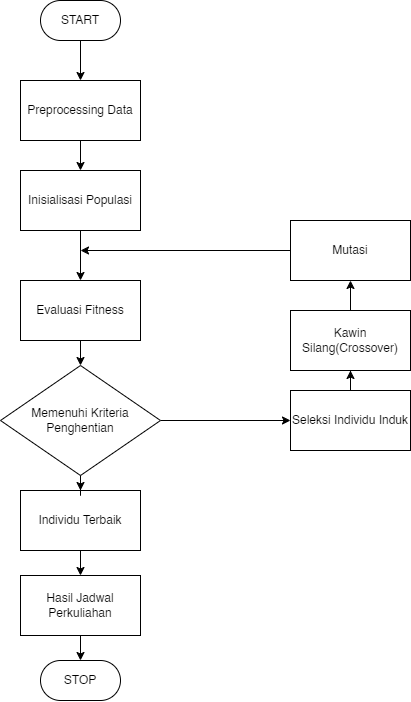
\includegraphics[scale=0.45]{gambar/Algoritma.png}
  % Keterangan gambar yang diinputkan
  \caption{Metodologi}
  % Label referensi dari gambar yang diinputkan
  \label{fig:Blueprint}
\end{figure}

% Contoh penggunaan referensi dari gambar yang diinputkan
Penulis akan menggunakan beberapa metode untuk menyelesaikan penelitian tersebut. 
Metode yang digunakan sebagai berikut:

\subsection{\emph{Preprocessing Data}}
  
  Pada penelitian ini, penulis akan menggunakan data dari Departemen Teknik Komputer ITS yang meliputi data mata kuliah, 
  jumlah ruangan, kapasitas masing-masing ruangan, jumlah dosen, dan jumlah mahasiswa. Data-data tersebut kemudian diolah 
  sedemikian rupa dengan metode encoding sehingga dihasilkan kromosom-kromosom yang akan digunakan sebagai induk dalam proses algoritma genetika.
  
\subsection{Inisialisasi Populasi}
  
  Individu-individu baru akan dibuat secara acak sesuai dengan desain kromosom yang telah dibuat sebelumnya.
  
  \subsection{Evaluasi Fitness}
  
  Individu dievaluasi dengan fungsi tertentu untuk menentukan kecocokan dengan batasan yang telah ditentukan sebelumnya. 
  Batasan-batasan tersebut dibagi menjadi 2 jenis yakni \emph{Hard Constraint} dan \emph{Soft Constraint.}
 
  \subsection{Pemilihan Indiidu Induk}
  
  Individu-individu yang telah melalui proses evaluasi dipilih untuk dijadikan sebagai induk untuk proses crossover. 
  Untuk memilihnya, dihitung probabilitas masing-masing individu dari nilai fitnessnya, kemudian dirandom menggunakan metode \emph{Roullete Wheel.}
 
  \subsection{\emph{Crossover}}
  
  Gen pada kromosom induk yang telah dipilih dipindah-silangkan sebagian antara satu dengan yang lain sehingga dihasilkan individu baru.

  \subsection{Mutasi}
  
  Setelah terbentuk individu baru, dilakukan perhitungan probabilitas mutasi untuk menentukan individu dan gen mana yang akan dimutasi. 
  Hasil dari mutasi ini akan dievaluasi nilai fitness nya untuk melihat apakah telah memenuhi kriteria atau belum. Kemudian proses akan berjalan lagi dari awal hingga memenuhi kriteria penghentian.
  
  \subsection{Kriteria Penghentian}
  
  Proses algoritma genetika hanya akan berhenti jika telah memenuhi kriteria penghentian yang telah ditentukan sebelumnya. 
  Kriteria penghentian ini dapat berupa nilai fitness tertentu, atau jumlah tertentu. 
  Jika nilai fitness telah terpenuhi atau jumlah iterasi telah terlewati, maka proses algoritma genetika akan berhenti.

\section{Bahan dan peralatan yang digunakan}
Dalam penelitian ini akan digunakan beberapa perangkat yang dibutuhkan untuk menunjang berjalannya penelitian dengan baik.
Berikut merupakan hardware dan software yang digunakan dalam melakukan proses pembuatan program sekaligus pengujian program yang digunakan pada penelitian ini.
\subsection{\emph{Hardware}}
Perangkat komputer yang digunakan untuk pengerjaan tugas akhir ini adalah \emph{Asus TUF FX 505 DT} dengan spesifikasi \emph{AMD Ryzen 5 R5-3550H Processor, GeForce GTX 1650 Graphics, 8GB DDR4, 1TB HDD,} dan \emph{Windows 10 64-bit}.
\subsection{\emph{Software}}
\emph{Software} yang digunakan dalam penelitian ini adalah Microsoft Visual Studio.


\section{Urutan pelaksanaan penelitian}

% Ubah tabel berikut sesuai dengan isi dari rencana kerja
\newcommand{\w}{}
\newcommand{\G}{\cellcolor{gray}}
\begin{table}[h!]
  \captionof{table}{Tabel timeline}
  \label{tbl:timeline}
  \begin{tabular}{|p{3.5cm}|c|c|c|c|c|c|c|c|c|c|c|c|c|c|c|c|}

    \hline
    \multirow{2}{*}{Kegiatan} & \multicolumn{16}{|c|}{Minggu} \\
    \cline{2-17} &
    1 & 2 & 3 & 4 & 5 & 6 & 7 & 8 & 9 & 10 & 11 & 12 & 13 & 14 & 15 & 16 \\
    \hline

    % Gunakan \G untuk mengisi sel dan \w untuk mengosongkan sel
    Studi Literatur &
    \G & \G & \w & \w & \w & \w & \w & \w & \w & \w & \w & \w & \w & \w & \w & \w \\
    \hline

    Pengumpulan Data &
    \w & \G & \G & \w & \w & \w & \w & \w & \w & \w & \w & \w & \w & \w & \w & \w \\
    \hline

    Preprocessing Data &
    \w & \w & \G & \G & \G & \w & \w & \w & \w & \w & \w & \w & \w & \w & \w & \w \\
    \hline

    Pembuatan Program &
    \w & \w & \w & \w & \G & \G & \G & \G & \G & \G & \G & \G & \w & \w & \w & \w \\
    \hline

    Pengujian Program &
    \w & \w & \w & \w & \w & \w & \w & \w & \w & \w & \w & \G & \G & \G & \w & \w \\
    \hline

    Penyusunan \linebreak Laporan &
    \G & \G & \G & \G & \G & \G & \G & \G & \G & \G & \G & \G & \G & \G & \G & \G \\
    \hline

  \end{tabular}
<<<<<<< HEAD
  \captionof{table}{Tabel timeline}
  \label{tbl:timeline}
\end{table}
=======
\end{table}

Pada \emph{timeline} yang tertera di Tabel \ref{tbl:timeline} \lipsum[10]
>>>>>>> f57e126874d0e1c43c733bfa968b0cb0f430594e

  \newpage

  % Konten lainnya
  \chapter{HASIL YANG DIHARAPKAN}

\section{Hasil yang Diharapkan dari Penelitian}

Dari penelitian yang akan dilakukan, diharapkan jadwal perkuliahan dapat dihasilkan dan memenuhi 
batasan-batasan yang telah ditentukan dan sesuai dengan kebutuhan dari Departemen Teknik Komputer ITS.

\section{Hasil Pendahuluan}

Sampai saat ini, kami telah melakukan wawancara terhadap staff administrasi akademik prodi sarjana untuk mengetahui 
gambaran mengenai kondisi terkini dari penjadwalan di Departemen Teknik Komputer ITS.

  \newpage

  % Daftar pustaka
  \chapter*{DAFTAR PUSTAKA}
  \addcontentsline{toc}{chapter}{DAFTAR PUSTAKA}
  \renewcommand\refname{}
  \vspace{2ex}
  \renewcommand{\bibname}{}
  \begingroup
    \def\chapter*#1{}
    \printbibliography
  \endgroup


\end{document}
